%
% Modified by Sameer Vijay
% Last Change: Wed Jul 27 2005 13:00 CEST
%
%%%%%%%%%%%%%%%%%%%%%%%%%%%%%%%%%%%%%%%%%%%%%%%%%%%%%%%%%%%%%%%%%%%%%%%%
%
% Sample Notre Dame Thesis/Dissertation
% Using Donald Peterson's ndthesis classfile
%
% Written by Jeff Squyres and Don Peterson
%
% Provided by the Information Technology Committee of
%   the Graduate Student Union
%   http://www.gsu.nd.edu/
%
% Nothing in this document is serious except the format.  :-)
%
% If you have any suggestions, comments, questions, please send e-mail
% to: ndthesis@gsu.nd.edu
%
%%%%%%%%%%%%%%%%%%%%%%%%%%%%%%%%%%%%%%%%%%%%%%%%%%%%%%%%%%%%%%%%%%%%%%%%

%
% Chapter 2
%

\chapter{TRANSFER REACTIONS AND NUCLEAR MATRIX ELEMENTS}
\label{chap:nucl}

\section{Shell Model of the Nucleus}
\begin{comment}
Using H.O. eigenstates to describe nucleons.
\begin{itemize}
\item nuclear potential well - is this something we can understand independently?  Certainly the radius is.
\item solutions to finite square well in terms of H.O. eigenstates and a diagram of energy levels
\item the energy levels give correct shell closures when spin-orbit coupling is introduced
\item so H.O. eigenstates are a reasonable way to describe nucleons
\end{itemize}

Looking at the valence nucleons to understand the whole nucleus.
\begin{itemize}
\item and because the nucleons couple so strongly into \zp pairs, describing the unpaired nucleons often accurately describes the entire nucleus
\item give a simple example?  \He{3} might be useful?
\item show level filling for \Ge{74} (32 protons) and point out the valence nucleons are f, p, g
\end{itemize}
\end{comment}

Trends in systematic nuclear data such as nuclear mass gave clear evidence of ``magic numbers'' of protons and neutrons in nuclei, but it was not until Maria Goeppert-Mayer added a spin-orbit term to the HO potential that these magic numbers were correctly reproduced.  Describing a nucleus with more than three nucleons in any basis set would be an arduous task were it not for the surprisingly accurate assumption that closed shells in the nucleus form an inert core with $J=0$.  Furthermore, nucleons have a strong tendency to couple into $J=0$ pairs, so that to understand the behavior of the nucleus it is often sufficient to understand only the behavior of the unpaired nucleons.

The nucleus of primary interest in this work, \Se{76}, has 34 protons and 42 neutrons.  Like all even-even nuclei, its ground states is \zp, evidencing the strong coupling of nucleons into $J=0$ pairs.  The nucleons studied by ($^3$He,n) transfer are proton-pair holes; the valence shell of \GeTargets are shown in {\fig}~\ref{fig:valence}.  It is important to note that while the central potential with spin-orbit coupling accurately reproduces the magic numbers seen in nuclear data, it is by no means a universal potential that accurately describes all nuclei.  The exact energy levels in \GeTargets are not known, and so the valence shell is considered to be f-p-g rather than simply 1f$_{5/2}$.

\section{Nucleon States and the Impact they Have on NME}
\begin{comment}
\subsection{NME calculations and valence States}
\begin{itemize}
\item (assume that) NME calculations are sensitive to occupied valence states
\item can investigate valence state occupation with transfer reactions
\item \Ge{76} occupancies were experimentally determined and adjusting the energy levels to match changed the NME by a factor of 2 \cite{0vbbReview}
\end{itemize}
\end{comment}
As discussed in {\chap}~\ref{chap:0vbb}, the half-life of the \zvbb process depends on the nuclei as well as the neutrino mass scale.  While a direct measurement of \NME = $\langle f||O||i \rangle$ is difficult because it is only directly accessible by observation of \zvbb, it is possible to study the initial and final nuclear states separately in an attempt to improve the accuracy of the calculation.  Ambitious programs to study the initial- and final-state candidate nuclei via single-nucleon transfer have been underway since ?? [CITE].  Single-nucleon transfer is an important tool in understanding the occupancy of valence nucleons.  Very generally, the cross-section for transferring a nucleon to a specific state in a target nucleus will be high if that nucleus has many holes available in that state but low if that state in the nucleus is filled.  Single-nucleon transfer reactions (where a nucleon is transferred onto a target) can be used to form a picture of shell occupancy and vacancy within a nucleus.  The valence neutrons in the candidate nucleus \GeTargets and its daughter \SeProducts have been studied with the neutron-adding reactions (d,p) and ($\alpha$,\He{3}) as well as neutron-removing reactions (p,d) and (\He{3},$\alpha$) \cite{valenceNeutrons}.  The valence protons of these same nuclei have been studied with the (d,\He{3}) reaction \cite{valenceProtons}.  These studies demonstrated that the Fermi surface of both the protons and neutrons in \GeTargets are quite diffuse, with the relevant neutron and proton orbits being 1$p_{3/2}$, 0$f_{5.2}$, 1$p_{1/2}$, and 0$g_{9/2}$.  The quantities most important to the NME calculations are the differences in occupancies between the mother and daughter nucleus; these differences are shown in {\fig}~\ref{fig:occupancyDiffs} along with the theoretical predictions.
\begin{figure}[htp]
\centering
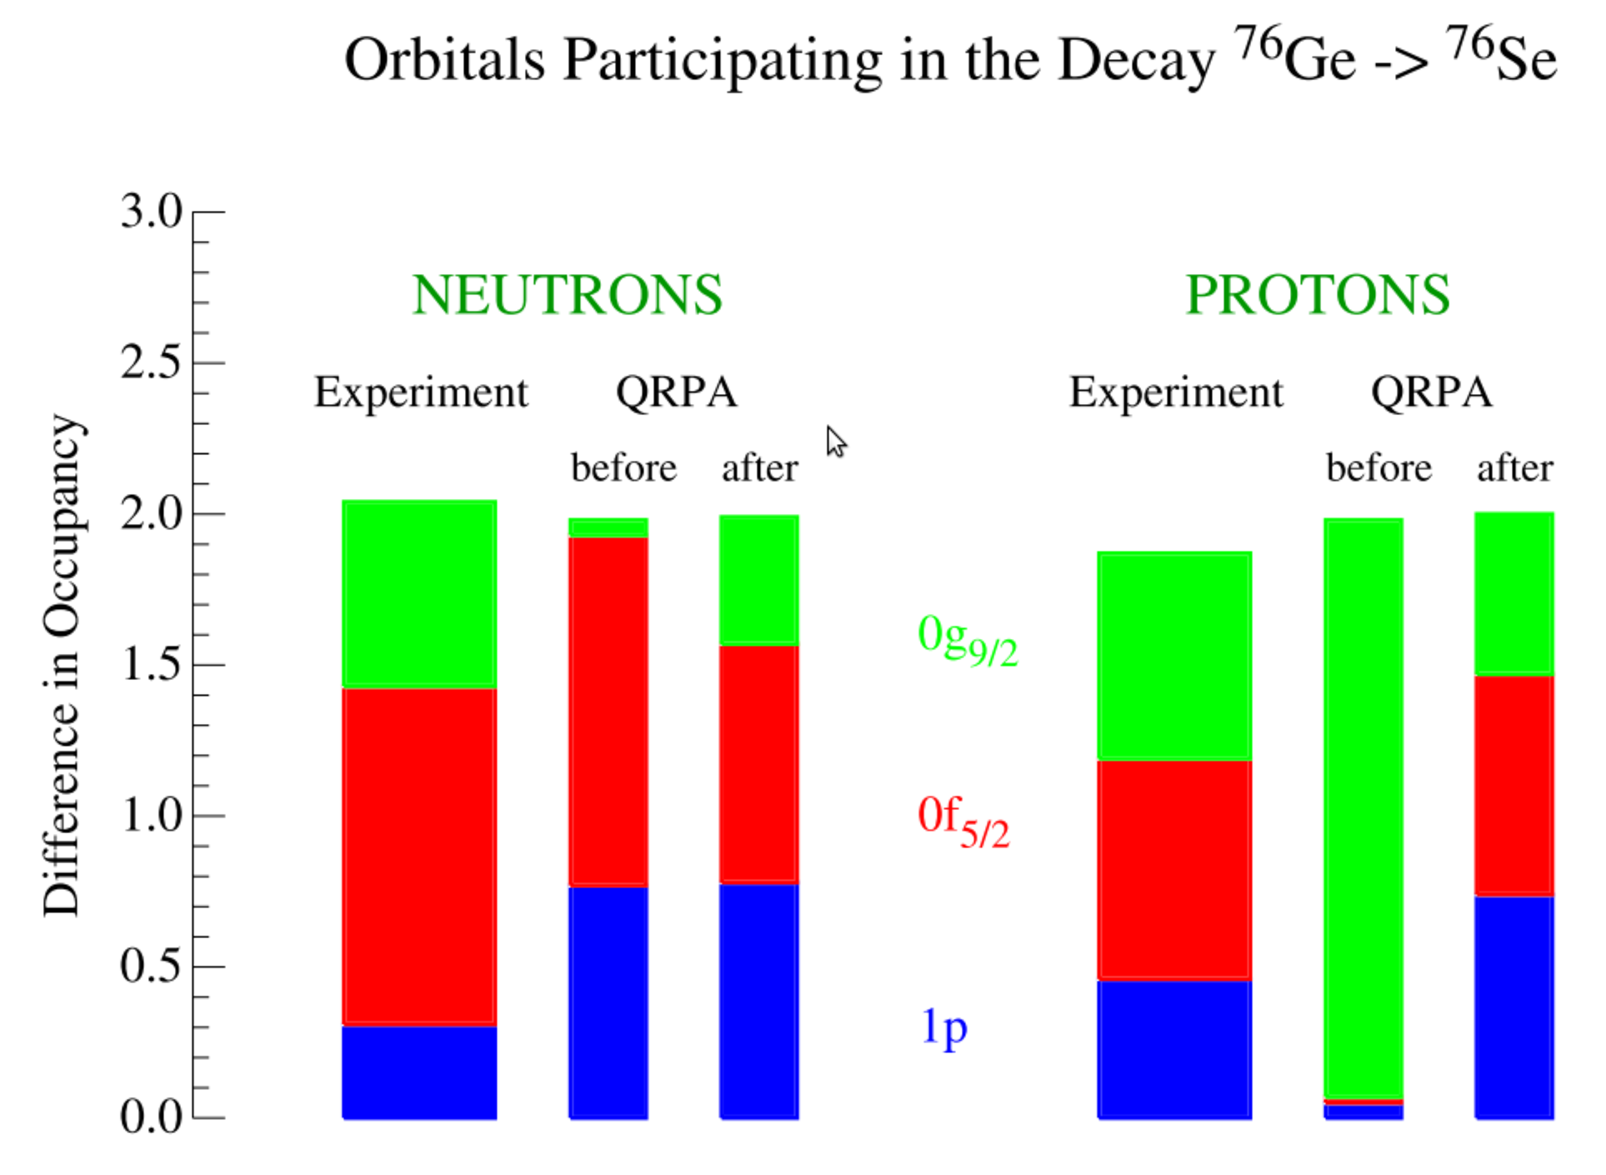
\includegraphics[width=1.0\textwidth]{figures/occupancyDiffs.eps}
\caption{From \cite{schiffer_review}.}
\label{fig:occupancyDiffs}
\end{figure}
The single-particle energy levels were adjusted in the QRPA calculation \cite{SuhonenEnergyAdjust} to provide better agreement with the data.  These changes reduced the QRPA calculation of \NME by approximately a factor of two, bringing it into agreement with the shell-model calculation of \NME.  This reduction in the spread of calculated \NME is particularly valuable to reducing the uncertainty of mass limits or estimates from \zvbb searches. 


\section{Nucleon-nucleon correlations and the impact they have on NME}
\begin{comment}
\begin{itemize}
\item \zvbb occurs on correlated neutron pairs
\item certain pairing in the nucleus can inhibit \zvbb
\item investigate pair correlation with two-nucleon transfer reactions
\item some systems don't have all their \zp in the ground state - Xe
\item discuss neutron transfer experiments done on \GeTargets
\item wish to investigate proton transfer on \GeTargets
\end{itemize}
\end{comment}
In addition to studying the single-nucleon states in \GeTargets and \SeProducts, understanding correlated neutron pairs in \Ge{76} and correlated proton pairs in \Se{78} is relevant to \NME.  Calculations suggest that significant contributions to \NME come from inter-nucleon distances of less than 3~fm \cite{anatomy}.  The distribution of highly-spatially-correlated \zp strength, therefore, may strongly influence \NME.  QRPA calculations can be particularly sensitive to \zp strength that is not exclusively in the ground state as these models assume a BCS approximation where the ground state contains all \zp strength [CITE]. 

Pair-transfer reactions such as (p,t) and (\He{3},n) are useful probes of pairing in nuclei as the cross-section for \zp states is dramatically forward peaked and therefore distinct \cite{Yoshida}.  The cross section of a two-nucleon transfer reaction on a nucleus that is well described by BCS should show strong population of the \zp ground-state with little, if any, population of \zp excited states.  A system that demonstrates the motivation for studying pairing in \Ge{74} particularly well is $^{128,130}$Te.  The neutron-pair adding reaction (p,t) was used to show that the cross section for excited \zp states is less than 4\% of that for the ground-state \zp cross section \cite{neutronPairsTellurium}, suggesting that BCS symmetry is a reasonable approximation for the neutrons in $^{128,130}$Te.  The same is not true for the proton states; the (\He{3},n) reaction populates an excited \zp state with a cross section that is $\sim$30\% of the ground-state cross section \cite{protonPairsTellurium}.  Studies of \Ge{76}(p,t) and \Se{76}(p,t) show that the \zp strength is distributed overwhelmingly to the ground state, with excited-\zp states being populated at less than a few percent \cite{neutronPairsGermanium}.  As can be seen in $^{128,130}$Te, however, \zp strength distribution of the neutrons in a nucleus is not necessarily that of the protons.  The aim of this work is to study the distribution of the proton-\zp strength using the two-proton transfer reaction \reaction.   

\section{Modeling Two-Proton Transfers}
\begin{comment}
Discuss DWBA theory of two-proton transfer reactions
\begin{equation}
M\sim\langle\psi_n|V_T|\psi_{^3He}\rangle
\end{equation}
Where $V_T$ is the transfer operator and $\psi$ are elastic scattering wave functions.
Assume that nuclear elastic scattering is the largest contribution to the nuclear reaction and use 1st order perturbation theory to generate $V_T$ from the bound-state wave functions.
To get $\psi$ (?)
\begin{enumerate}
\item treat two particles individually
\item treat two protons as bound cluster
\end{enumerate}
treating particles individually is too complicated
when using cluster model, can adjust $V_0$ of well to match ?? binding energy and adjust $r_0$ to adjust range and $a_0$ to adjust ??.

cluster model's prediction of 0 degree cross section is sensitive to these parameters, but the relative cross sections of f-p-g shell nuclei do not depend strongly on the parameters.

Discuss experimental difficulties of two-proton transfer reactions and introduce NSL as a good place to do them
\end{comment}
Measuring differential cross sections can give information about underlying characteristics of nuclei.  For example, population of excited \zp states in two-nucleon transfer reactions gives information about pairing in a nucleus.  However, cross sections are also influenced by factors not related to nuclear structure such as optical-model potentials.  These contributions are not as interesting as those that are sensitive to the pairing force.  The distorted-wave Born approximation (DWBA) is used to calculate cross sections of transfer reactions by assuming that nuclear elastic scattering is the largest contribution to the nuclear reaction and that the transfer operator can be constructed from the bound-state wavefunctions of the initial and final states using first-order perturbation theory.  This assumption is particularly accurate for the forward angles which are of interest in this experiment.

In general, four potentials are needed to perform a DWBA calculation in the case of a transfer reaction $(A = C+x)+B\rightarrow C+(D = B+x)$ where $x$ is transferred onto the nucleus $B$.  The potential felt by incoming nucleus $A$ due to nucleus $B$ and the potential felt by the outgoing nucleus $C$ due to the product nucleus $D$ are both necessary.  The optical-model potentials are of the form
\begin{equation}
U(r) = V_C - Vf(x_0) + \left( \frac{h}{m_{\pi}c} \right) ^2 V_{SO}(\sigma\cdot l)\frac{1}{r}\frac{d}{dr}f(x_{SO})
-i[Wf(x_W) - 4W_D\frac{d}{dx_D}f(x_D)],
\end{equation}
where $V_C$ is the coulomb potential and $f(x)=(1+e^x)^{-1}$ is the Woods-Saxon potential \cite{PereyPerey}.  The variable $x$ is defined as $(r-r_iA^{1/3})/a_i$, where $r$ is the distance from the center of the nucleus, $r_i$ is the characteristic radius of a particular interaction, and $a_i$ describes the diffuseness.  Note that the functional form of the spin-orbit term $V_{SO}(\sigma\cdot l)$ is the derivative of the Woods-Saxon potential, making it predominantly a surface effect.  The imaginary component of the potential allows for absorbtion and, like the real part, has a volume term $W$ and a surface term $W_D$.  Potentials to bind the transfer nucleus (or nucleon) to its original nucleus $C$ and final nucleus $B$ are also needed. 
When calculating proton-pair transfer cross sections, this method can be complicated considerably when treating each proton in the pair separately.  This approach is that of Bayman and Kallio [CITE] and can sometimes accurately predict the absolute differential cross section.  A simpler method, the cluster model, treats the protons as a single, bound cluster.  While this method does not typically reproduce absolute cross sections well, it reproduces the angular distribution of the more-complicated Bayman-Kallio approach.  It should be noted that when using the either model to predict cross sections, their magnitude is quite sensitive to the parameters in the Woods-Saxon potential, $r$ and $a$, which describe the radius of the well and the diffuseness of the surface, respectively.  However, the trend of the cross-section relative to the energy of the incoming \He{3} or changing neutron number of the target is well-reproduced.

One can use DWBA calculations to understand the kinematic dependence of the expected cross section as in {\fig}~\ref{fig:optimizeCrossSection}; this helps determine an appropriate beam energy.  
\begin{figure}[htp]
\centering
\includegraphics[width=1.0\textwidth]{figures/74Ge_0plus_xsection.eps}
\caption{A plot showing the $^{74}$Ge($^3$He,n) \zp cross section at zero degrees as a function of beam energy.  From ??.}
\label{fig:optimizeCrossSection}
\end{figure}
It can be seen from this plot that the ideal beam energy for maximizing the \reaction cross section is slightly more than 18~MeV.  However, detector resolution decreases with increasing beam energy as discussed in {\sect}~\ref{sec:detector}.  Because the product nuclei \SeProducts have low-lying excited \tp states that could be populated with similar cross section to the ground state, the lower beam energy of 16~MeV was chosen to provide sufficient resolution for resolving these states.  See {\fig}~\ref{fig:levelDiagrams} for level diagrams of the product nuclei.
\begin{figure}[!htbp]
\centering
\subfloat[][]{
   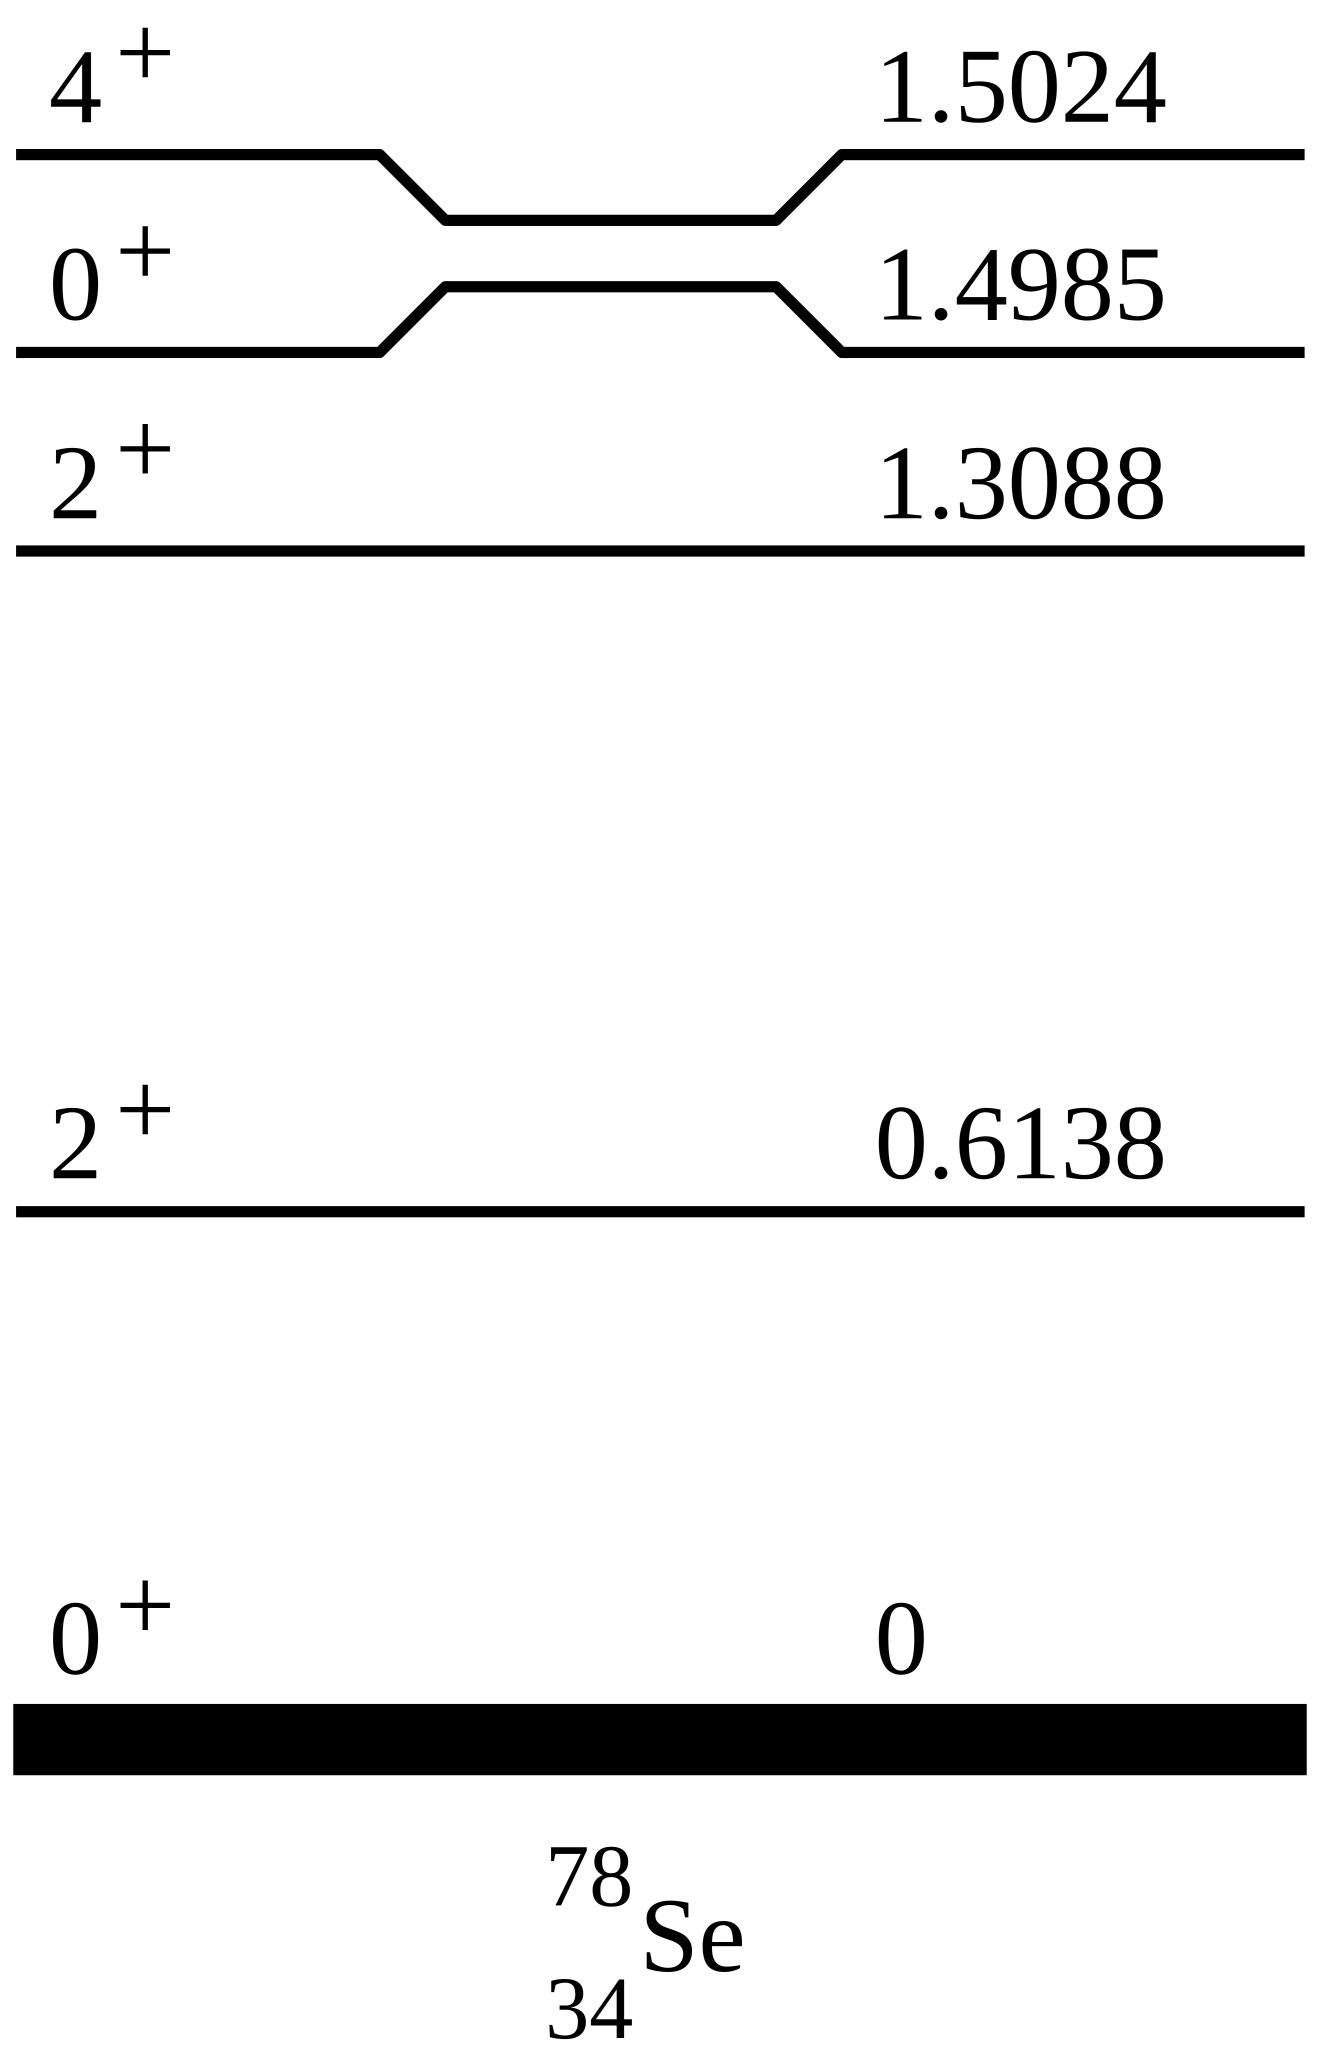
\includegraphics[width=0.3\textwidth]{figures/78Ge_levels.eps}
}
\subfloat[][]{
   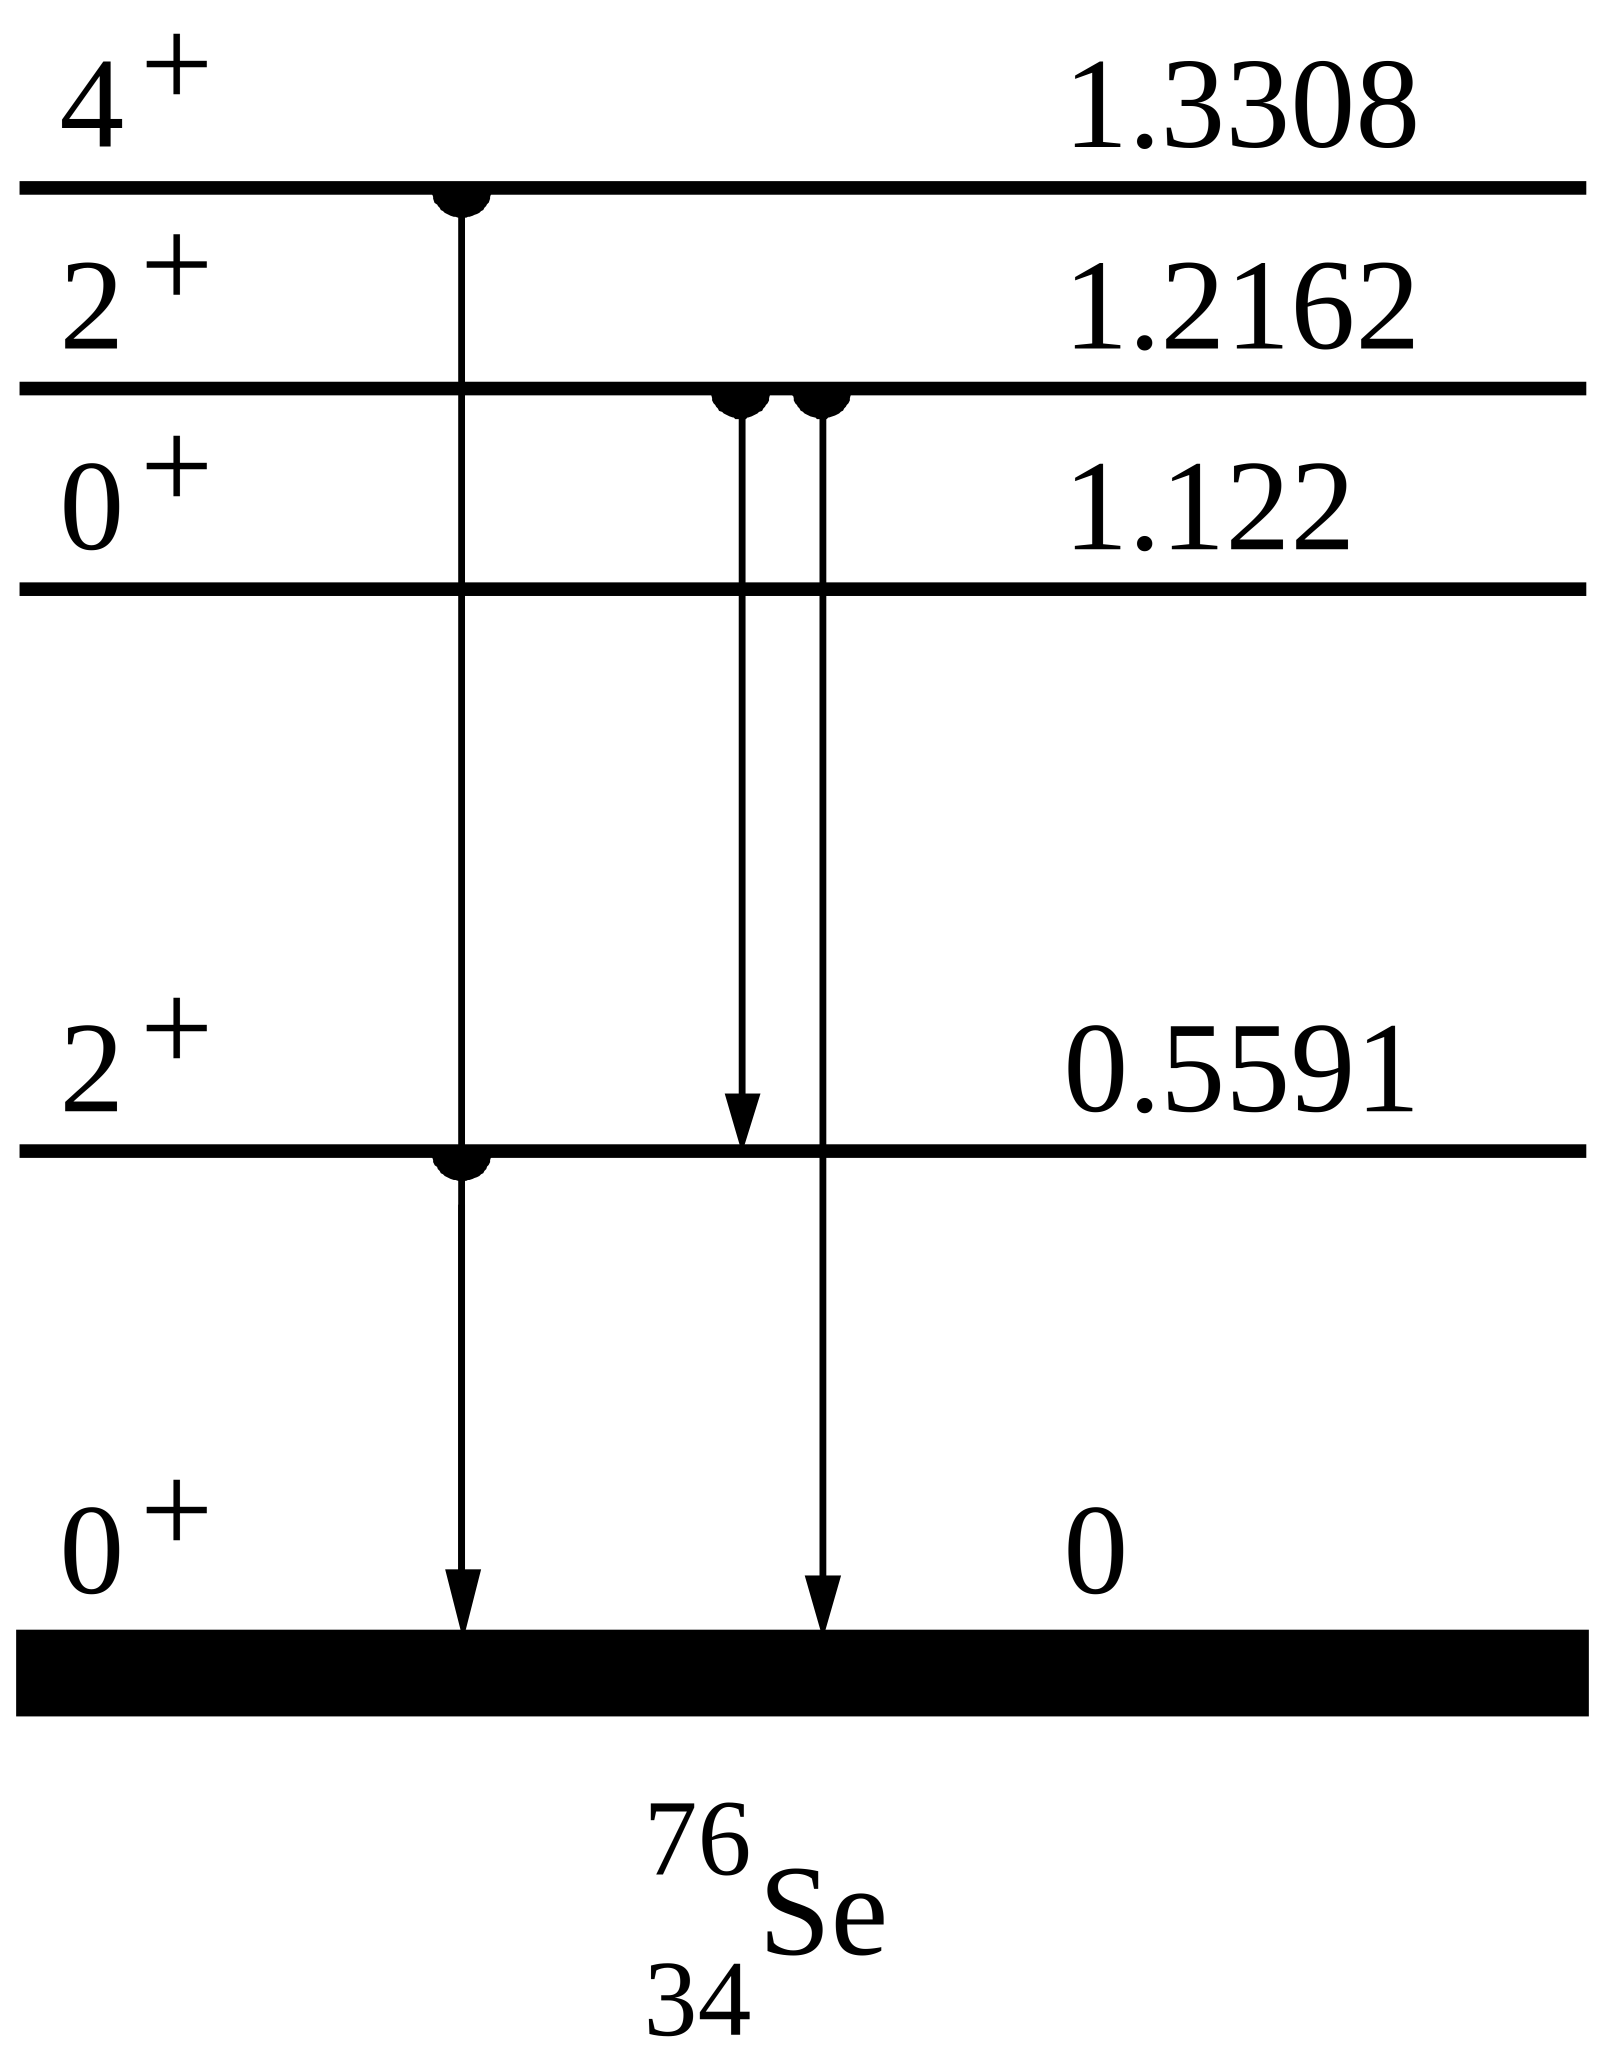
\includegraphics[width=0.3\textwidth]{figures/76Ge_levels.eps}
}
\caption{The level diagrams of the product nuclei, \Se{78} and \Se{76}.  Note the low-lying 2$^+$ state.  Notice also that both nuclei have known \zp levels.  These levels have been measured through $\gamma$-ray experiments.  Such experiments are not sensitive to the pairing in ground-state nuclei, which is why two-nucleon transfer reactions on \zvbb candidate nuclei are of such interest.}
\label{fig:levelDiagrams}
\end{figure}
Particulars of the beam and neutron detector are discussed in {\chap}~\ref{chap:2pExpt} and an analysis of the results in {\chap}~\ref{chap:dataAnalysis}.
% % uncomment the following lines,
% if using chapter-wise bibliography
%
% \bibliographystyle{ndnatbib}
% \bibliography{example}
